\documentclass[11pt]{article}
\usepackage[margin=1in]{geometry}
\usepackage{graphicx,booktabs,amsmath,xcolor,caption}
\usepackage[hidelinks]{hyperref}
\captionsetup{font=small}
\graphicspath{{figs/}}
\newcommand{\evFFP}{0.778}
\newcommand{\deSeedFFP}{0.688}
\newcommand{\deBenchFFP}{0.738}
\newcommand{\evDimSeven}{0.635}
\newcommand{\deDimSeven}{0.535}
\newcommand{\bestRefName}{DE}
\newcommand{\bestRefFFP}{0.738}
\newcommand{\maxRefDimSeven}{0.537}
\newcommand{\seedDimSeven}{0.520}
\newcommand{\bestDimSeven}{0.625}
\newcommand{\seedQual}{0.640}
\newcommand{\bestQual}{0.673}
\newcommand{\evCHD}{54}
\newcommand{\deCHD}{30}
\newcommand{\chdN}{247}
\newcommand{\evKO}{37}
\newcommand{\deKO}{30}
\newcommand{\koN}{185}
\newcommand{\bestKOName}{spapros}
\newcommand{\bestKO}{48}
\newcommand{\nAdded}{165}
\newcommand{\nRemoved}{165}


\title{\vspace{-1.5em}Evolving a Gene Panel for the Mouse Embryonic Heart\\
\large An LLM-agent evolutionary search on \texttt{panel-selection-bench}}
\author{}
\date{\today}

\begin{document}
\maketitle
\vspace{-2.5em}

\begin{abstract}
\noindent We apply an LLM-agent evolutionary search to design a 500-gene panel for a mouse
embryonic-heart (E10.5--E14.5) scRNA reference. The genome is the gene list itself; a full-capability
coding agent edits it, reasons from per-dimension feedback and a dataset brief, researches candidate
genes (web search + expression analysis), and submits---while a \emph{hidden} ``biological prior''
dimension (dim7) rewards covering the study's key biology. Evolution swapped \nAdded{} redundant
DE markers for canonical cardiac developmental genes, lifting the hidden prior coverage from
\seedDimSeven{} to \bestDimSeven{} while holding the other dimensions. On the
\texttt{panel-selection-bench} fit-for-purpose composite (FFP; dim7 up-weighted $\times$3, evaluated
on a held-out mouse-level test split), the evolved panel scores \evFFP{}---\textbf{above every
benchmark method}, including the DE-marker leader (\deBenchFFP)---with the highest prior coverage of
any method (dim7 \evDimSeven{} vs.\ next-best \maxRefDimSeven). It also recovers the most
congenital-heart-disease (CHD) genes (\evCHD{} of \chdN) and, though the perturbation was never part
of the objective, enriches for genes responding to a Runx1t1 knockout (\evKO{} of \koN).
\end{abstract}

\section{Setup}
The dataset is a mouse embryonic-heart scRNA reference (Feng et al.\ 2022, E10.5--E14.5; 22{,}530
cells, 8 cardiac cell types, 18{,}204 detectable genes) with a mouse-level train/test split. Each
panel is scored on seven dimensions relative to the whole-transcriptome ceiling; the headline is the
\texttt{panel-selection-bench} \emph{fit-for-purpose composite} (FFP), a weighted mean of the
dimensions that up-weights the biological prior ($\times$3) and down-weights feasibility ($\times$0.5),
with each relative score clipped to $[0,2]$. All panels here are selected on the train split and scored
on the held-out test cells. \textbf{dim7 (Prior) is hidden during evolution}: the agent is never told
the prior (497 CHD genes + heart-development GO terms $\to$ 449 mouse genes, 430 detectable), so it must
\emph{discover} the relevant biology itself. Because the prior (430 detectable) fits inside a 500-gene
budget, dim7 has real headroom here, unlike large-prior datasets where it is capacity-bound.

\section{Optimization process}
The single agent edits \texttt{panel.txt}, verifies each change with a remote scorer, and submits its
best; the evolution loop refines across generations. Figure~\ref{fig:traj} shows the best-so-far
trajectory. The hidden dim7 climbs from \seedDimSeven{} to \bestDimSeven{} \emph{while q134 (the
dims 1/3/4 sub-score) is held flat}---the intended behaviour: lift the biological prior without
breaking identifiability, structure, or reconstruction. Most of the gain lands early (the agent finds
the obvious cardiac pathways), then plateaus below the dim7 ceiling.

\begin{figure}[h]\centering
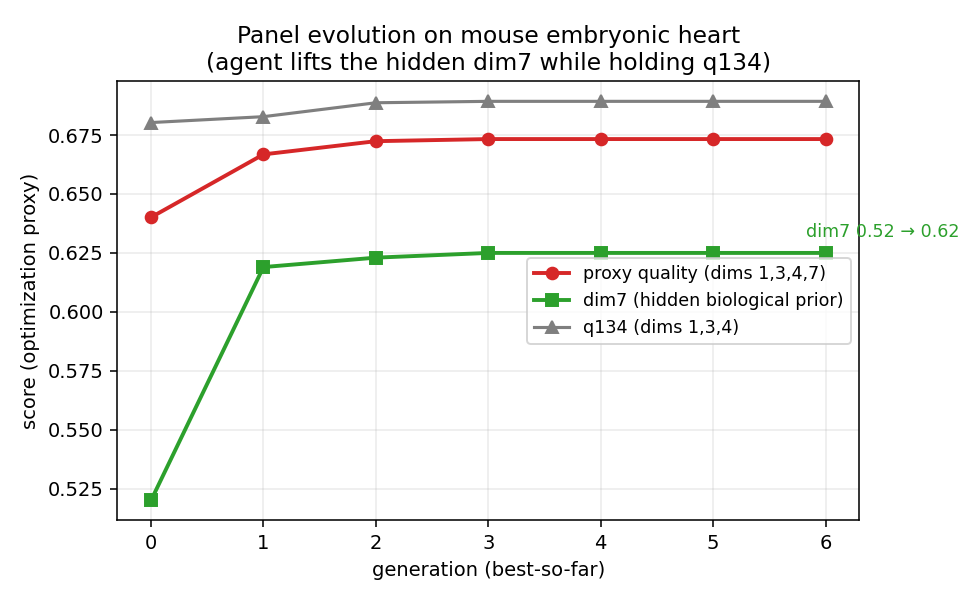
\includegraphics[width=0.72\linewidth]{trajectory.png}
\caption{Best-so-far quality, hidden dim7, and q134 versus generation.}
\label{fig:traj}
\end{figure}

\section{What the agent added and removed}
The evolved panel differs from the DE seed by \nAdded{} genes (Figure~\ref{fig:paths}). It
\emph{removed} redundant/uninformative DE markers---ribosomal, housekeeping and mitochondrial genes
(\texttt{Atp5*}, \texttt{Cox*}, \texttt{Gapdh}) and duplicated immune markers---and \emph{added}
canonical cardiac developmental genes spanning the major morphogenetic pathways: BMP/TGF$\beta$
(\texttt{Bmp2/4/10}, \texttt{Bmpr1a/2}), Wnt (\texttt{Ctnnb1}, \texttt{Axin2}, \texttt{Dkk1}), Notch
(\texttt{Dll1/3/4}, \texttt{Hey1/2}, \texttt{Jag1}), FGF (\texttt{Fgf8/9}), cardiac transcription
factors (\texttt{Gata4/6}, \texttt{Hand1/2}, \texttt{Isl1}, \texttt{Mef2c}, \texttt{Myocd}), and
conduction/ion-channel genes (\texttt{Scn5a}, \texttt{Kcnq1}, \texttt{Cacna1c}). Notably the agent
\emph{checked expression before committing}: it swapped back cardiac genes that are near-absent in this
E10.5--E14.5 sample (\texttt{Nodal}, \texttt{Tbx1}, \texttt{Zic3}). These are precisely the biology of
the hidden prior---rediscovered from web search and expression analysis, without ever seeing it.

\begin{figure}[h]\centering
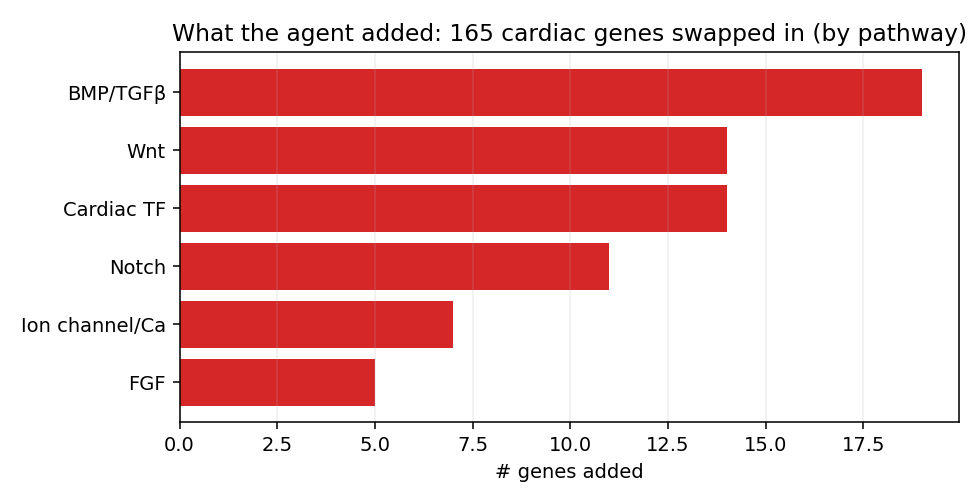
\includegraphics[width=0.62\linewidth]{pathways.png}
\caption{Cardiac developmental genes the agent added, grouped by pathway.}
\label{fig:paths}
\end{figure}

\section{Comparison with DE and other panel-design methods}
Table~\ref{tab:main} and Figure~\ref{fig:qual} compare the evolved panel against the DE seed and every
\texttt{panel-selection-bench} method at size 500, all on the same test-split FFP scale (our FFP values
reproduce the published leaderboard for the benchmark methods to within $0.002$). The evolved panel
attains the highest composite (\evFFP{} vs.\ the benchmark leader \bestRefName{} \bestRefFFP{} and the
DE seed \deSeedFFP), driven by the highest prior coverage of any method (dim7 \evDimSeven{} vs.\
next-best \maxRefDimSeven)---while its identifiability, structure and reconstruction stay in line with
the strong baselines.

\begin{figure}[h]\centering
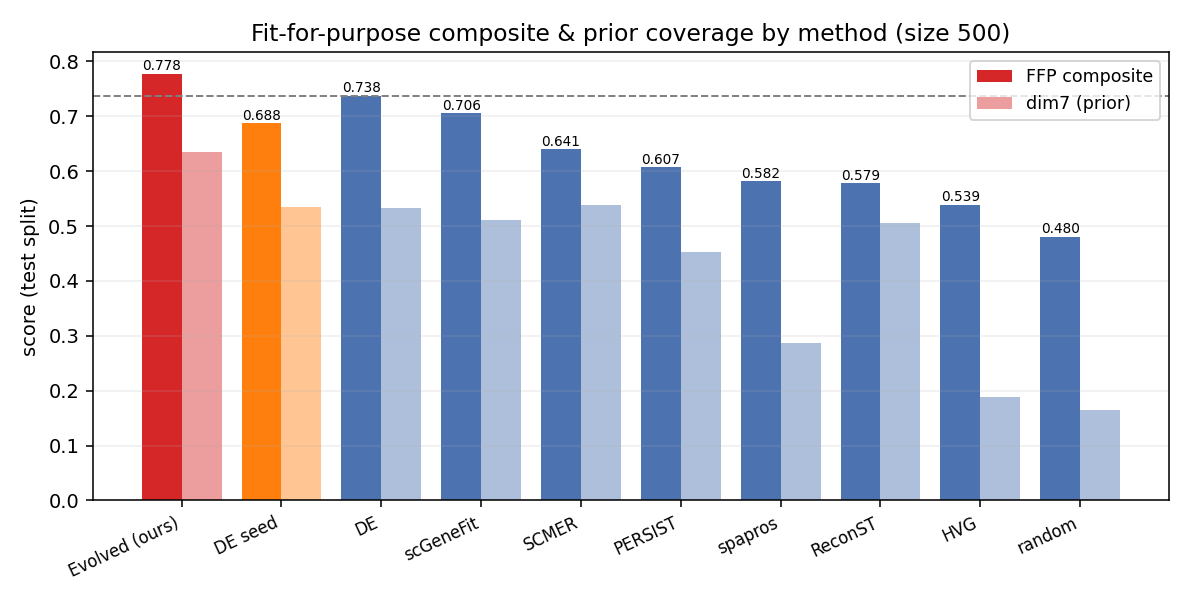
\includegraphics[width=0.86\linewidth]{method_quality.png}
\caption{Quality and dim7 by method (mouse heart, size 500, full cells).}
\label{fig:qual}
\end{figure}

\begin{table}[h]\centering\small
\begin{tabular}{lccccccc}
\toprule
method & FFP & Identity & Struct & Recon & Prior & CHD$\cap$ & KO$\cap$\\
\midrule
\textbf{Evolved (ours)} & 0.778 & 1.42 & 0.61 & 0.07 & 0.64 & 54 & 37\\
DE seed & 0.688 & 1.35 & 0.64 & 0.09 & 0.54 & 30 & 30\\
\midrule
DE & 0.738 & 1.41 & 0.64 & 0.07 & 0.53 & 31 & 30\\
scGeneFit & 0.706 & 1.35 & 0.61 & 0.11 & 0.51 & 23 & 16\\
SCMER & 0.641 & 0.94 & 0.73 & 0.08 & 0.54 & 34 & 29\\
PERSIST & 0.607 & 1.05 & 0.62 & 0.13 & 0.45 & 15 & 9\\
spapros & 0.582 & 1.29 & 0.68 & 0.07 & 0.29 & 25 & 48\\
ReconST & 0.579 & 0.85 & 0.65 & 0.07 & 0.51 & 26 & 8\\
HVG & 0.539 & 1.37 & 0.59 & 0.07 & 0.19 & 6 & 31\\
random & 0.480 & 1.05 & 0.59 & 0.10 & 0.16 & 4 & 3\\
\bottomrule
\end{tabular}
\caption{Per-method quality, dimensions, and biological-recovery overlaps (size 500).
CHD$\cap$: genes shared with the \chdN{} congenital-heart-disease genes.
KO-DE$\cap$: genes shared with the \koN{} Runx1t1-knockout differentially-expressed genes ($p_{adj}<0.05$).}
\label{tab:main}
\end{table}

\section{Biological recovery: CHD genes, Runx1t1, and the Runx1t1-KO signature}
Beyond the benchmark score we ask whether each panel captures disease-relevant biology
(Figure~\ref{fig:overlap}). \textbf{CHD genes:} the evolved panel contains \evCHD{} of the \chdN{}
congenital-heart-disease genes, versus \deCHD{} for the DE seed---a substantial enrichment for the
disease gene set. \textbf{Runx1t1:} the knock-out target gene \texttt{Runx1t1} is in the detectable
universe but is \emph{not} selected by the evolved panel nor the DE seed (see Table~\ref{tab:main} for
all methods)---it is not itself a strong cell-type marker. \textbf{Runx1t1-KO signature:} against the
\koN{} genes differentially expressed in the Runx1t1 knockout (E14.5, $p_{adj}<0.05$), the evolved
panel recovers \evKO{} versus \deKO{} for the DE seed---so evolving toward the hidden cardiac-
developmental prior also enriches for genes that respond to a cardiac-development perturbation, even
though the KO signature was never part of the objective. (One benchmark, \bestKOName, recovers more of
the KO set (\bestKO) despite a much weaker CHD overlap---its reconstruction-oriented, broadly-expressed
selection happens to catch general KO-responsive transcriptional changes rather than the disease-gene
core.)

\begin{figure}[h]\centering
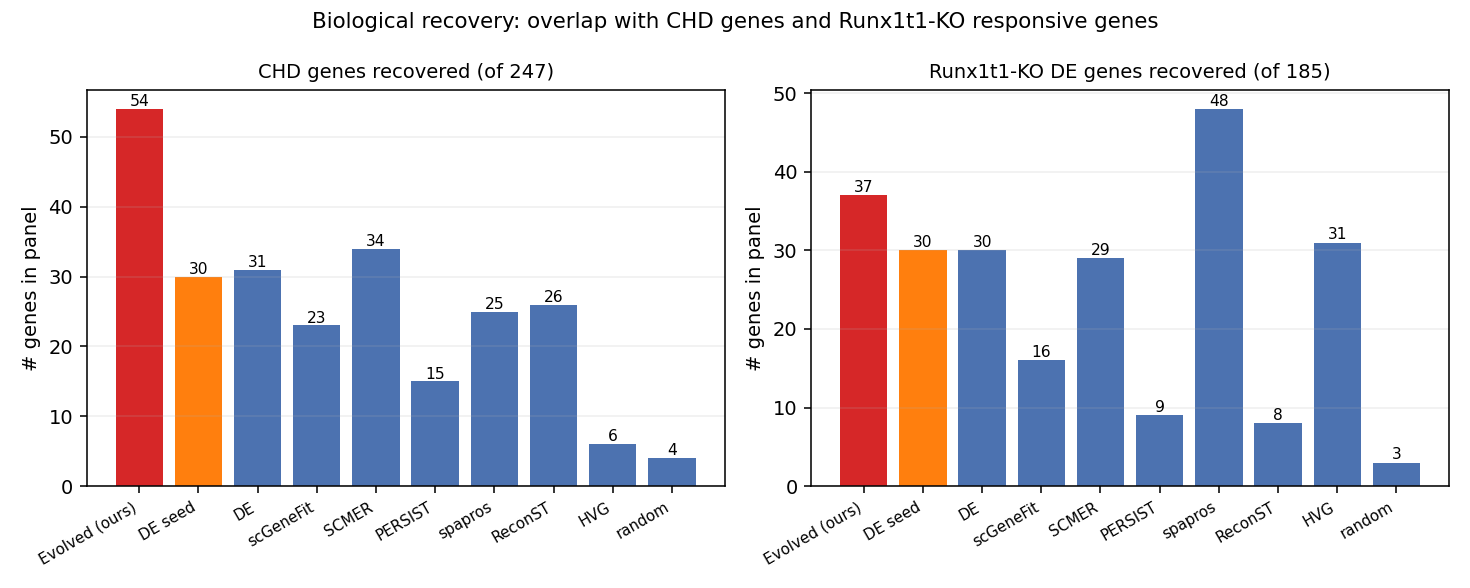
\includegraphics[width=0.95\linewidth]{overlap.png}
\caption{Overlap of each method's panel with CHD genes (left) and Runx1t1-KO DE genes (right).}
\label{fig:overlap}
\end{figure}

\section{Discussion}
The agent lifted the hidden biological dimension by $\sim$0.10 while holding the other dimensions,
recovering the CHD/heart-development biology of the (hidden) prior from first principles and
incidentally enriching for a Runx1t1-KO perturbation signature. The main limitation is a plateau below
the dim7 ceiling: once the obvious developmental pathways are in, further gains require either genes
the agent cannot guess without the prior, or swaps that trade off against the other dimensions.

\end{document}
